% Preambel mit Einstellungen importieren
\input{tex/preambel}

% Dokumenteninfos importieren
% -------------------------------------------------------
% Daten für die Arbeit
% Wenn hier alles korrekt eingetragen wurde, wird das Titelblatt
% automatisch generiert. D.h. die Datei titelblatt.tex muss nicht mehr
% angepasst werden.

\newcommand{\dhbwsprache}{en} % de oder en für Deutsch oder Englisch
                              % Für korrekt sortierte Literatureinträge, noch preambel.tex anpassen

% Titel der Arbeit auf Deutsch
\newcommand{\dhbwtitelde}{Deep Learning Based Object Classification on Edge Devices}

% Titel der Arbeit auf Englisch
\newcommand{\dhbwtitelen}{Deep Learning Based Object Classification on Edge Devices}

% Weitere Informationen zur Arbeit
\newcommand{\dhbwort}{Mannheim}    % Ort
\newcommand{\dhbwautorvname}{Koen} % Vorname(n)
\newcommand{\dhbwautornname}{Logmann} % Nachname(n)
\newcommand{\dhbwcoautorvname}{Jessica} % Vorname(n)
\newcommand{\dhbwcoautornname}{Roth} % Nachname(n)
\newcommand{\dhbwdatum}{\today} % Datum der Abgabe
\newcommand{\dhbwjahr}{2019} % Jahr der Abgabe
\newcommand{\dhbwfirma}{SAP SE, Walldorf} % Firma bei der die Arbeit durchgeführt wurde
\newcommand{\dhbwbetreuer}{Prof. Dr. Ivo Wolf, Hochschule Mannheim} % Betreuer an der Hochschule
\newcommand{\dhbwzweitkorrektor}{Dr. Julien Vayssiere, SAP SE} % Betreuer im Unternehmen oder Zweitkorrektor
\newcommand{\dhbwfakultaet}{I} % I für Informatik
\newcommand{\dhbwstudiengang}{AI} % IB IMB UIB IM MTB

% Zustimmung zur Veröffentlichung
\setboolean{dhbwpublizieren}{true}   % Einer Veröffentlichung wird zugestimmt
\setboolean{dhbwsperrvermerk}{false} % Die Arbeit hat keinen Sperrvermerk

% -------------------------------------------------------
% Abstract

% Kurze (maximal halbseitige) Beschreibung, worum es in der Arbeit geht auf Deutsch
\newcommand{\dhbwabstractde}{Die Hauptthematik der vorliegenden Masterarbeit umfasst den Vergleich zwischen Edge Devices und Cloud Services für die Objektklassifizierung mittels Deep Learning. Die grundlegende Fragestellung dabei ist, welches die beste Arbeitsumgebung dafür bildet. Um diese Frage zu erörtern ist es notwendig, zu Beginn geeignete Netzwerke zu finden und diese auf den Probanten optimal zu installieren und zu trainieren. Mittels der experimentellen Methode werden folgend alle Netzwerke auf den Edge Devices und auf den Cloud Services getestet und evaluiert. Die daraus resultierenden Ergebnisse werden untereinander verglichen und mittels einer gewichteten Entscheidungsmatrix bewertet. Entgegen dem aktuellen Trend zu den Cloud Services hin, zeigten die Ergebnisse des Vergleichs eine Daseinsbereichtigung der Edge-Devices und eine Empfehlung hin zu diesen aufgrund mehrerer serverseitiger Probleme im Umgang mit den Cloud Services. }

% Kurze (maximal halbseitige) Beschreibung, worum es in der Arbeit geht auf Englisch

\newcommand{\dhbwabstracten}{The main topic of this master thesis is the comparison between Edge Devices and Cloud Services for object classification using Deep Learning. The basic question is which of the two variants represents the best working environment for this. In order to discuss this question, it is necessary to find suitable networks at the beginning and to install and train them optimally on the test equipment. Using the experimental method, all networks on the edge devices and cloud services will be tested and evaluated. The results are compared with each other and evaluated using a weighted decision matrix. Contrary to the current trend towards cloud services, the results of the comparison showed that the Edge devices were in the same category and a recommendation for them due to several server-side problems in dealing with cloud services for specific applications.}



% Literatur-Datenbank
\addbibresource{literatur.bib}   % BibLaTeX-Datei mit Literaturquellen einbinden

\begin{document}
\frontmatter

% Römische Ziffern für die "Front-Matter"
\setcounter{page}{0}
\changefont{ptm}{m}{n}  % Times New Roman für den Fließtext
\renewcommand{\rmdefault}{ptm}

% Titelblatt
% -------------------------------------------------------
% In dieser Datei sollten eigentlich keine Veränderungen mehr
% notwendig sein.
% -------------------------------------------------------

\thispagestyle{empty}

% Fakultäten der DHBW-Mannheim
% -------------------------------------------------------
\ifthenelse{\equal{\dhbwfakultaet}{I}}%
  {\newcommand{\dhbwfakultaetlangde}{Fakultät für Informatik}%
   \newcommand{\dhbwfakultaetlangen}{Department of Computer Science}}{}

\ifthenelse{\equal{\dhbwfakultaet}{E}}%
  {\newcommand{\dhbwfakultaetlangde}{Fakultät für Elektrotechnik}%
   \newcommand{\dhbwfakultaetlangen}{Department of Electrical Engineering}}{}

\ifthenelse{\equal{\dhbwfakultaet}{S}}%
  {\newcommand{\dhbwfakultaetlangde}{Fakultät für Sozialwesen}%
   \newcommand{\dhbwfakultaetlangen}{Department of Social Work}}{}



\ifthenelse{\equal{\dhbwstudiengang}{IB}}%
  {\newcommand{\dhbwstudienganglangde}{Informatik}%
  \newcommand{\dhbwstudienganglangen}{Computer Science}%
  \newcommand{\dhbwtypde}{Bachelor-Thesis}%
  \newcommand{\dhbwtypen}{Bachelor Thesis}%
  \newcommand{\dhbwgrad}{\dhbwbsc}}{}
  
\ifthenelse{\equal{\dhbwstudiengang}{AI}}%
  {\newcommand{\dhbwstudienganglangde}{Angewandte Informatik}%
  \newcommand{\dhbwstudienganglangen}{Applied Computer Science}%
  \newcommand{\dhbwtypde}{Bachelor-Thesis}%
  \newcommand{\dhbwtypen}{Bachelor Thesis}%
  \newcommand{\dhbwgrad}{\dhbwbsc}}{}

\ifthenelse{\equal{\dhbwstudiengang}{SAB}}%
  {\newcommand{\dhbwstudienganglangde}{Soziale Arbeit}%
   \newcommand{\dhbwstudienganglangen}{Social Labour}%
   \newcommand{\dhbwtypde}{Bachelor-Thesis}%
   \newcommand{\dhbwtypen}{Bachelor Thesis}%
   \newcommand{\dhbwgrad}{\dhbwba}}{}
   
\ifthenelse{\equal{\dhbwstudiengang}{SAM}}%
  {\newcommand{\dhbwstudienganglangde}{Soziale Arbeit}%
   \newcommand{\dhbwstudienganglangen}{Social Labour}%
   \newcommand{\dhbwtypde}{Master-Thesis}%
   \newcommand{\dhbwtypen}{Master Thesis}%
   \newcommand{\dhbwgrad}{\dhbwmastera}}{}

\ifthenelse{\equal{\dhbwstudiengang}{TIB}}%
  {\newcommand{\dhbwstudienganglangde}{Technische Informatik}%
   \newcommand{\dhbwstudienganglangen}{Technical Information Technology}%
   \newcommand{\dhbwtypde}{Bachelor-Thesis}%
   \newcommand{\dhbwtypen}{Bachelor Thesis}%
   \newcommand{\dhbwgrad}{\dhbwbsc}}{}
  

\newcommand{\dhbwbsc}{Bachelor of Science (B.Sc.)}
\newcommand{\dhbwba}{Bachelor of Arts (B.A.)}
\newcommand{\dhbwmaster}{Master of Science (M.Sc.)}
\newcommand{\dhbwmastera}{Master of Arts (M.A.)}
\newcommand{\dhbwmasterba}{Master of Business Administration (MBA)}

\newcommand{\dhbwkoerperschaftde}{DHBW Mannheim}
\newcommand{\dhbwkoerperschaften}{Baden-Wuerttemberg Cooperative State University Mannheim}

\newcommand{\dhbwautorbib}{\dhbwautornname, \dhbwautorvname \  \& \dhbwautorrnname, \dhbwautorrvname} % Autor Nachname, Vorname
\newcommand{\dhbwautor}{\dhbwautorvname \ \dhbwautornname \  \& \dhbwautorrvname \ \dhbwautorrnname} % Autor Vorname Nachname

\ifthenelse{\equal{\dhbwsprache}{de}}%
  {\newcommand{\dhbwtyp}{\dhbwtypde}%
   %\newcommand{\dhbwthesistype}{zur Erlangung des akademischen Grades \dhbwgrad}%
   \newcommand{\dhbwthesistype}{Studienarbeit}%
   \newcommand{\dhbwkoerperschaft}{\dhbwkoerperschaftde}%
   \newcommand{\dhbwstudiengangname}{Studiengang \dhbwstudienganglangde}%
   \newcommand{\dhbwstudienganglang}{\dhbwstudienganglangde}%
   \newcommand{\dhbwtitel}{\dhbwtitelde}%
   \newcommand{\dhbwtutor}{Betreuer}%
   \newcommand{\dhbwfakultaetlang}{\dhbwfakultaetlangde}%
   \newcommand{\dhbwlistoftables}{Tabellenverzeichnis}%
   \newcommand{\dhbwlistoffigures}{Abbildungsverzeichnis}%
   \newcommand{\dhbwlistings}{Quellcodeverzeichnis}%
   \newcommand{\dhbwindex}{Index}%
   \newcommand{\dhbwabbreviations}{Abkürzungsverzeichnis}%   
   \selectlanguage{ngerman}}
   %else
  {\newcommand{\dhbwtyp}{\dhbwtypen}%
   %\newcommand{\dhbwthesistype}{for the acquisition of the academic degree \dhbwgrad}%
   \newcommand{\dhbwthesistype}{T\_3200}%
   \newcommand{\dhbwkoerperschaft}{\dhbwkoerperschaften}%
   \newcommand{\dhbwstudiengangname}{Course of Studies: \dhbwstudienganglang}%
   \newcommand{\dhbwstudienganglang}{\dhbwstudienganglangen}%
   \newcommand{\dhbwtitel}{\dhbwtitelen}%
   \newcommand{\dhbwtutor}{Tutors}
   \newcommand{\dhbwfakultaetlang}{\dhbwfakultaetlangen}%
   \newcommand{\dhbwlistoftables}{List of Tables}%
   \newcommand{\dhbwlistoffigures}{List of Figures}%
   \newcommand{\dhbwlistings}{Listings}%
   \newcommand{\dhbwindex}{Index}%
   \newcommand{\dhbwabbreviations}{List of Abbreviations}%
   \selectlanguage{english}}%


% Daten in die Standard-Felder von KOMA-Script eintragen
\titlehead{\dhbwtyp\ in\  \dhbwstudienganglang}
\subject{}
\title{\dhbwtitel}
\author{\dhbwauthor}
\date{\small{\dhbwdatum}}

% Daten für das fertige PDF-Dokument
\hypersetup{
  pdftitle={\dhbwtitel},  % Titel des Dokuments
  pdfauthor={\dhbwautor},              % Autor
  pdfsubject={\dhbwtyp\ in\ \dhbwstudienganglang},                % Thema
  pdfkeywords={\dhbwtitel}         % Schlüsselworte
}

\newlength{\bindekorrektur}
\newlength{\seitenanfang}
\newlength{\seitenbreite}
  
\setlength{\bindekorrektur}{-46mm}   % Korrektur der horizontalen Position
\setlength{\seitenanfang}{0mm}       % Korrektur der vertikalen Position
\setlength{\seitenbreite}{297mm}

%\noindent\includegraphics[width=7cm]{dhbw-logo.pdf}\\
\noindent\includegraphics[width=0.49\textwidth]{img/DHBW-Logo.pdf}
\hfill
%\noindent\includegraphics[width=0.27\textwidth]{SAP_grad_R_pref.png}

% Titel der Arbeit
\begin{textblock*}{128mm}(45mm,\seitenanfang + 62mm) % 4,5cm vom linken Rand und 6,0cm vom oberen Rand
  \centering\Large\sffamily
  \vspace{4mm} % Kleiner zusätzlicher Abstand oben für bessere Optik
  \textbf{\dhbwtitel}
\end{textblock*}%

% Name
\begin{textblock*}{128mm}(45mm,\seitenanfang + 103mm)
  \centering\large\sffamily
  \dhbwautor
\end{textblock*}

% Thesis
\begin{textblock*}{\seitenbreite}(\bindekorrektur,\seitenanfang + 130mm)
  \centering\large\sffamily
  %\dhbwtyp\\
  Study report \\ %TODO only for this thesis
  \begin{small}\dhbwthesistype \end{small}\\
  \vspace{2mm}
  \dhbwstudiengangname
\end{textblock*}

% Fakultät
\begin{textblock*}{\seitenbreite}(\bindekorrektur,\seitenanfang + 165mm)
  \centering\large\sffamily
  \dhbwfakultaetlang\\
  \vspace{2mm}
  \dhbwkoerperschaft
\end{textblock*}

% Datum
\begin{textblock*}{\seitenbreite}(\bindekorrektur,\seitenanfang + 190mm)
  \centering\large 
  \textsf{\dhbwdatum}
\end{textblock*}

% Firma
\begin{textblock*}{\seitenbreite}(\bindekorrektur,\seitenanfang + 215mm)
  \centering\large 
  %\textsf{Durchgeführt bei der Firma \dhbwfirma}
\end{textblock*}

% Betreuer
\begin{textblock*}{\seitenbreite}(\bindekorrektur,\seitenanfang + 240mm)
  \centering\large\sffamily
  \dhbwtutor \\
  \vspace{2mm}
  \dhbwbetreuer\\
  \vspace{2mm}
  \dhbwzweitkorrektor
\end{textblock*}

% Bibliographische Informationen
\null\newpage
\thispagestyle{empty}
  
\newcommand{\dhbwbibde}{\begin{small}\textbf{\dhbwautorbib}: \\ \dhbwtitelde \ / \dhbwautor. \ -- \\ \dhbwtypde, \dhbwort : \dhbwkoerperschaftde, \dhbwjahr. \pageref{lastpage} Seiten.\end{small}}

\newcommand{\dhbwbiben}{\begin{small}\textbf{\dhbwautorbib}: \\ \dhbwtitelen \ / \dhbwautor. \ -- \\ \dhbwtypen, \dhbwort : \dhbwkoerperschaften, \dhbwjahr. \pageref{lastpage} pages. \end{small}}

\ifthenelse{\equal{\dhbwsprache}{de}}%
  {\dhbwbibde \\ \vspace{0.5cm} \\ \dhbwbiben}
  {\dhbwbiben \\ \vspace{0.5cm} \\ \dhbwbibde}


% Erklärung
\clearpage\setcounter{page}{1}
\thispagestyle{empty}
\textsf{\large\textbf{Erklärung}}

Hiermit erkläre ich, dass ich die vorliegende Arbeit selbstständig verfasst und keine anderen als die angegebenen Quellen und Hilfsmittel benutzt habe.

\ifthenelse{\boolean{dhbwpublizieren} \and \not\boolean{dhbwsperrvermerk}}%
{
\vspace{0.5cm}
Ich bin damit einverstanden, dass meine Arbeit veröffentlicht wird, d.\,h. dass die Arbeit elektronisch gespeichert, in andere Formate konvertiert, auf den Servern der Hochschule Mannheim öffentlich zugänglich gemacht und über das Internet verbreitet werden darf. 
}{}%


\vspace{1cm}
\dhbwort, \dhbwdatum \\

\vspace{1.2cm}						                                      
\dhbwautor

\ifthenelse{\boolean{dhbwsperrvermerk}}%
{%
\vspace{11cm}
\color{red}\textsf{\large\textbf{Sperrvermerk}}

Diese Arbeit basiert auf internen und vertraulichen Daten des Unternehmens \dhbwfirma.

Diese Arbeit darf Dritten, mit Ausnahme der betreuenden Dozenten und befugten Mitglieder des Prüfungsausschusses, ohne ausdrückliche Zustimmung des Unternehmens und des Verfassers nicht zugänglich gemacht werden.

Eine Vervielfältigung und Veröffentlichung der Arbeit ohne ausdrückliche Genehmigung -- auch in Auszügen -- ist nicht erlaubt.
\color{black}
}{}

\cleardoublepage

% Abstract
\chapter*{Abstract}

\ifthenelse{\equal{\dhbwsprache}{de}}%
  {\subsubsection*{\dhbwtitelde}\dhbwabstractde\subsubsection*{\dhbwtitelen}\dhbwabstracten}
  {\subsubsection*{\dhbwtitelen}\dhbwabstracten\subsubsection*{\dhbwtitelde}\dhbwabstractde}



% Inhaltsverzeichnis erzeugen
\cleardoublepage
\pdfbookmark{\contentsname}{Contents}
\tableofcontents

% Korrigiert Nummerierung bei mehrseitigem Inhaltsverzeichnis
\cleardoublepage
\newcounter{frontmatterpage}
\setcounter{frontmatterpage}{\value{page}}

% Arabische Zahlen für den Hauptteil
\mainmatter

% Den Hauptteil mit vergrößertem Zeilenabstand setzen
\onehalfspacing

% ------------------------------------------------------------------
% Hauptteil der Arbeit
    % !TeX root = ./documentation.tex

\chapter{Introduction}
\section{Motivation}
\section{Objective of the work}
Die Aufgabenstellung dieser Studienarbeit handelt von der Animation des Davis Putman Algorithmus anhand des N Damen Problems mit der Hilfe von Javascript. Dabei werden mehrere Kriterien definiert, die diese Animation erfüllen muss, da sie vor allem zur Visualisierung und zur genaueren anschaulichen Verdeutlichung beziehungsweise Erklärung des Algorithmus dient. Die genauen Anforderungen werden im Laufe dieser Arbeit genauer spezifiziert und am Ende am finalen Produkt evaluiert. Der Hauptteil dieser Arbeit handelt deshalb von der Konzeption und der Implementierung dieser Aufgabenstellung.
%TODO Koen: Fällt dir noch etwas dazu ein?
\section{Structure of the report}
Um die Navigation durch diese Arbeit zu erleichtern, wird im folgenden Abschnitt einen kurzen Blick in die Struktur dieser Arbeit geworfen. 
\\
Im nächsten Kapitel werden die mathematischen Grundlagen zum Davis Putman Algorithmus und des N Damen Problems geschaffen. Dabei handelt es sich vor allem um die logischen Zusammenhänge und der mathematisch korrekten Definition des zu lösenden Problems. 
\\
Darauffolgend wird im dritten Kapitel ein allgemeiner Überblick zu den verwendeten Bibliotheken und Technologien gegeben und Hintergrundinformationen geliefert, aus welchen Gründen bestimmte Technologien bevorzugt beziehungsweise ausgewählt wurden.
\\
Im vierten Abschnitt dieser Arbeit wird die Konzeption des Programms genauer betrachtet. Vor allem handelt es von der allgemeinen Architektur und dem erstellten Layout Design, das als Vorlage für die Implementierung der Benutzeroberfläche dient. Eingeleitet wird das Kapitel durch das Spezifizieren der Anforderungen für das Programm, die eine zentrale Rolle in der Evaluation am Ende spielen.
\\
Im fünften Kapitel wird nun Schritt für Schritt durch die fertige Implementierung geleitet und der Aufbau des Programms genauer erläutert. Dabei wird durch die unterschiedlichen Komponenten und Klassen geführt und dabei ihre Funktion genauer erläuert.
\\
Das letzte Kapitel wird mit der Evaluation der Anforderungen begonnen. Dies dient vor allem dazu, um zu schauen, ob das Programm alle Kriterien erfüllt und zu Ende als erfolgreich erfüllt angesehen werden kann. Danach folgt ein zusammenfassendes Fazit und ein Ausblick, wie das Programm zukünftig weiterentwickelt oder anders eingesetzt werden könnte.
    % !TeX root = ../documentation.tex

% Davis Putnam in own word

\chapter{Scientific Basics}
% cSpell:disable
% Das Ziel dieser Arbeit besteht in der Visualisierung des Davis Putman Algorithmus, der das sogenannte N damen Problem lösen soll. Dafür muss zuerst ein allgemeines Verständnis zu diesem Algorithmus und dem mathematischen Problem geschaffen werden. In diesem Kapitel wird aus diesem Grund dieses fundamentale Wissen zusammengefasst, um eine Basis für die weiterführende Entwicklung zu schaffen. Dafür spielt unter anderem die Deklarierung des mathematischen Problems eine Rolle, damit dieses vom Davis Putman Algorithmus gelöst werden kann.
% cSpell:enable
The purpose of this work is to visualize the Davis Putman algorithm solving the so-called \textit{N-Queens Problem}. 
Therefore a general understanding of this algorithm and the mathematical problem has to be created.

This chapter summarizes the fundamental knowledge that is needed in order to create a basis for further development. 
%TODO: rephrase following sentence:
Among other things, the definition of the mathematical problem plays a role here, so that it can be solved by the Davis Putman algorithm.

\section{The Algorithm of Davis \& Putnam}
% cSpell:disable
% Der Davis Putman Algorithmus ist ein Verfahren zur Berechnung einer Lösung von aussagelogischen Klauselmengen. Bei sehr kleinen Klauselmengen kann dies leicht bestimmt werden, wie in den zwei folgenden Beispielen zu sehen ist.
% cSpell:enable
The Davis Putman algorithm is a method for calculating a solution a set of propositional clauses. With very small clause sets this can be easily determined, as can be seen in the following two examples.
\\
\hspace*{1.3cm} 
$K_1 = \bigl\{\; \{r\},\; \{\neg s\},\; \{t\},\; \{\neg u\}, \; \{\neg v\} \;\bigr\}$ 
\\[0.2cm]
$K_1$
% cSpell:disable
%kann auch als aussagelogische Formel geschrieben werden.
% cSpell:enable
can also be written as a propositional logic formula.
\\[0.2cm]
\hspace*{1.3cm}
$r \land \neg s \land t \land \neg u \land \neg v$.
\\[0.2cm]
% cSpell:disable
% Es ist erkennbar, dass diese Formel lösbar ist, indem $r$ und $t$ \enquote{wahr} und $s$, $u$ und $v$ den Wert \enquote{falsch} haben. Als Gegenbeispiel dazu ist $K_2$ zu betrachten.
% cSpell:enable
It is recognizable that this formula is solvable by $r$ and $t$ \enquote{true} and $s$, $u$ and $v$ having the value \enquote{false}.
As a counter example $K_2$ is to be considered.
\\
\hspace*{1.3cm}
$K_2 = \bigl\{\; \{r\},\; \{\},\; \{t\} \;\bigr\}$ 
\\[0.2cm]
$K_2$ can also be written as a propositional logic formula.
\\[0.2cm]
\hspace*{1.3cm}
$r \land \bot \land t$.
\\[0.2cm]
% cSpell:disable
% Eine leere Klammer bedeutet in der Aussagelogik ein Falsum, wodurch $K_2$ unerfüllbar ist. Bei sehr großen Klauselmengen ist es meist nicht mehr auf dem ersten Blick zu sehen, so dass Algorithmen wie dieser eingesetzt werden. Doch um nun einen Schritt tiefer setzen zu können, müssen zwei Definitionen zuvor eingeführt werden.
% cSpell:enable
The empty set in the set of clauses $K_2$ is interpreted as a $\bot$ in the propositional logic, making it impossible to satisfy $K_2$. It is possible to satisfy smaller sets of less complex clauses by first glance, but it gets more difficult for larger and complexer sets of clauses. For these algorithms like the Davis Putman algorithm are used.
% TODO: rephrase following sentence:
But to be able to set a step lower, two definitions have to be introduced first. \cite{Zhang2000}

\paragraph{Unit clause}
% cSpell:disable
% Eine Klausel $C$ ist eine Unit-Klausel, wenn diese nur aus einem Literal, also aus einer Aussagevariablen besteht.
% cSpell:enable
A clause $C$ is a unit clause if it consists of only one literal, i.e. a variable or a negated variable.

\paragraph{trivial clause sets}
% cSpell:disable
% Eine triviale Klauselmenge kann nur vorkommen, wenn einer der beiden Fälle eintritt.
% cSpell:enable
A trivial set of clauses can only occur if one of the following two cases occurs.

\begin{enumerate}
% cSpell:disable
% $K$ enthält die leere Klausel und ist somit unerfüllbar
% cSpell:enable
\item A set of clauses $K$ contains the empty set and is therefore unsatisfiable
% cSpell:disable
% Die Unit-Klauseln beinhalten immer verschiedene Aussagevariablen, so dass entweder nur die Klausel $\{p\}$ oder $\{\neg p\}$ vorkommen kann. Ist dies der Fall, kann eine Lösung für die Klauselmenge bestimmt werden.
% cSpell:enable
\item The unit clauses always contain different statement variables, so that only the clause $\{p\}$ or $\{\neg p\}$ can occur. If this is the case, a solution for the clause set can be determined.
\end{enumerate}

% cSpell:disable
% Damit einer dieser beiden Fälle nun eintreten kann, müssen die Klauselmengen mit der Hilfe folgender drei Möglichkeiten so vereinfacht werden, dass diese nur aus Unit-Klauseln bestehen.
% cSpell:enable
In order for one of these two cases to occur, the clause sets must be simplified with the help of the following three options so that they consist only of unit clauses.

\begin{enumerate}
\item Cut Rule 
\item Subsumption
\item Case Differentiation
\end{enumerate}

% TODO: continue here
\subsection{Simplification with the Cut Rule} 
To simplify a set of clauses $K$ with $C_1 \cup \{\; p\; \}\, C_2 \cup \{\; \neg p\; \} \in K$ the cut rule can be used. Lets say we have two clauses $C_1$, $C_2$ and a variable $p$. A typical application of the cut rule is.
\\
\hspace*{1.3cm}
$\dfrac{C_1 \cup \{\; p\; \} \;\;\;\;\;\; C_2 \cup \{\; \neg p\; \}}{C_1 \cup C_2}$
\\[0.2cm]
In this case the result clause will in general have more literals than $C_1 \cup \{\; p\; \}$ or $C_2 \cup \{\; \neg p\; \}$ alone. Because if the clause $C_1 \cup \{\; p\; \}$ contains $m + 1$ literals and $C_1 \cup \{\; p\; \}$ contains $n + 1$ literals, then the union $C_1 \cup C_2$ can have upto $m + n$ literals in total. In general $m + n$ is bigger than $m + 1$ or $n + 1$. The clause can be smaller than previously if both sets contain the same literals, but it is only granted to be smaller if $m = 0 \lor n = 0$. This is the case for unit clauses. Therefore we will only allow the use of the cut rule if one of the clauses is a unit clause. These cuts will be called unit cuts. To be able to do those unit cuts with a unit clause $\{\; l\; \}$ on all clauses of a set of clauses $K$, we define the function
\\
\hspace*{1.3cm}
$\texttt{unitCut}: 2^{K} \times L \to 2^{K}$
\\[0.2cm]
so that for a set of clauses $K$ and a literal $l$ the function $\texttt{unitCut}(K,\; l)$ will simplify the set of clauses as much as possible by using unit cuts:
\\
\hspace*{1.3cm}
$\texttt{unitCut}(K,\; l) = \{\; C \setminus \{\; \neg l\; \}\; |\; C \in K\; \}$
\\[0.2cm]
The result set of clauses will have the same amount of clauses as $K$. Only the clauses $C \in K$ where $\neg l \in C$ were affected and got that element removed. \cite{Stroetman2019}

\subsection{Simplification with Subsumption}
For further simplification of the set of clauses we will use subsumption. The idea is simple and can be shown with the following example:
\\
\hspace*{1.3cm}
$K = \{\; \{\; l,\; p,\; \neg q \;\},\; \{\; l\; \}\; \} \cup M$
\\[0.2cm]
It is clear that the clause $\{\; l\; \}$ implies the clause $\{\; l,\; p,\; \neg q \;\}$, because if $\{\; l\; \}$ is satisfied, then $\{\; l,\; p,\; \neg q \;\}$ will be satisfied too. That's because
\\
\hspace*{1.3cm}
$\models l \to l \lor p \lor \neg q$
\\[0.2cm]
is given. With that in mind we can say that we can subsume a clause $C$ with a unit clause $U$ if $U \subseteq C$. That means if we have a set of clauses $K$ with $C \in K \land U \in K$ and $U$ can subsume $C$, we can remove the clause $C$ from $K$ to reduce its size. We define a function
\\
\hspace*{1.3cm}
$\texttt{subsume}: 2^{K} \times L \to 2^{K}$
\\[0.2cm]
that receives a set of clauses $K$ and a literal $l$. It will simplify $K$ by subsuming with the unit clause $\{\; l\; \}$:
\\
\hspace*{1.3cm}
$\texttt{subsume}(K,\; l) = \{\; C \in K\; |\; l \notin C\} \cup \{\{\; l\; \}\}$
\\[0.2cm]
We have to add the unit clause to the set of clauses, because $l \in U$ is the case. Resulting in $U$ being removed from $K$ at first too. \cite{Stroetman2019}

\subsection{Simplification with Case Differentiation}
% cSpell:disable
% Die Basis für das Prinzip der Fallunterscheidung bildet folgender Satz.
% cSpell:enable
The following theorem forms the basis for the principle of case differentiation.

\paragraph{Theorem}
% cSpell:disable
% Die Klauselmenge K ist genau dann erfüllbar, wenn die Klausel $K \cup \bigl\{\{p\}\bigr\}$ oder $K \cup \bigl\{\{\neg p\}\bigr\}$ erfüllbar ist.
% cSpell:enable
The set of clauses $K$ can only be satisfied if $K \cup \bigl\{\{p\}\bigr\}$ or $K \cup \bigl\{\{\neg p\}\bigr\}$ can be satisfied.

% cSpell:disable
% Für die Vereinfachung wird zu Beginn also eine Aussagenvariable p ausgewählt, die in der Klauselmenge vorkommt. Danach werden die beiden oben genannten Klauselmengen gebildet und versucht, für eine der beiden eine Lösung zu finden. Ist dieser Versuch erfolgreich, ist das Ergebnis automatisch die Lösung von $K$. Falls keine gefunden wird, ist $K$ unlösbar.
% TODO: Keine Ahnung ob hier Beweis einfügen soll
% cSpell:enable
For simplification, a statement variable p is selected at the beginning, which occurs in the clause set. Then the two clause sets mentioned above are formed and an attempt is made to find a solution for one of them. If this attempt is successful, the result is automatically a solution of $K$. If none is found, $K$ is unsolvable.

\subsection{The Davis-Putnam Method}
% cSpell:disable
% Durch die Wissensgrundlage, die zuvor geschaffen wurde, ist es nun möglich, das Vorgehen des Davis Putman Algorithmus zu skizzieren. Mit der Hilfe der Schnittregel und der Subsumption wird die Klauselmenge $K$ soweit es möglich ist, vereinfacht. Falls bereits nach diesem Schritt $K$ trivial ist, ist das Verfahren beendet. Andernfalls wird eine aussagelogische Variable p ausgewählt, die in K vorkommt. Dann wird rekursiv versucht, die Klauselmenge $K \cup \bigl\{\{p\}\bigr\}$ zu lösen, um eine Lösung für K zu finden. Wenn auch hier keine Lösung gefunden wurde, wird dasselbe mit dem negierten $p$ versucht. Scheitert auch dieser Versuch, ist K unlösbar.
% cSpell:enable
The theoretical foundation that was previously created now makes it possible to sketch the procedure of the Davis Putman algorithm. With the help of the intersection rule and the subsumption, the clause set $K$ is simplified as far as possible. If already after this step $K$ is trivial, the procedure is finished. Otherwise a statement logical variable p is selected, which occurs in K. Then a recursive attempt is made to solve the clause set $K \cup \bigl\{\{p\}\bigr\}$ in order to find a solution for K. If no solution was found here either, the same is tried with the negated $p$. If this attempt also fails, K is unsolvable.\cite{Zhang2000}, \cite{Stroetman2019}
% TODO: find more sources

% TODO: nicely format
\begin{listing}[ht]
function Satisfiable( clause set $S$ ) return boolean\\
  /* unit propagation */\\
  repeat for each unit clause $L$ in $S$ do\\
    /* unit subsumption */\\
    delete from $S$ every clause containing $L$\\
    /* unit resolution */\\
    delete $L$ from every clause of $S$ in which it occurs\\
  od\\
  if $S$ is empty then\\
    return true\\
  else if a clause becomes $\{\}$ in $S$ then\\
    return false\\
  fi\\
  until no further changes result\\
  /* splitting */\\
  choose a literal $L$ occurring in $S$\\
  if Satisfiable ($S \cup \{\{\neg L\}\}$) then\\
    return true\\
  else if Satisfiable ($S \cup \{\{L\}\}$) then\\
    return true\\
  else\\
    return false\\
  fi\\
end function
  \caption{A simple Davis–Putnam algorithm \cite{Zhang2000}}
  \label{listing:1}
\end{listing}  


\section{N Queens Problem}
% cSpell:disable
% Das n Königinnen Problem ist das verallgemeinerte mathematische Problem bezogen auf ein Schachbrett, dass n \times n Felder besitzt. Ein spezielles Beispiel dazu wäre das 8 Damen Problem, welches auf dem standardisierten Schachbrett abgebildet wird. Allgemein handelt das Problem davon, n Damen auf einem n \times n Schachbrett so zu platzieren, dass keine in ihrem Zug behindert werden würde. Eine Königin in einem normalen Schachspiel kann sowohl diagonal, als auch vertikal und horizontal ihre Züge ziehen. Dieses Zugmuster kann in Figure \ref{fig:queens-problem} genauer angeschaut werden. Zusammengefasst heißt dies also, dass immer nur eine Dame auf ihrer vertikalen, horizontalen und diagonalen Linie sein darf, um sich nicht gegenseitig zu behindern. Dabei wird in diesem Problem davon ausgegangen, dass jede Dame jede andere angreifen kann und die Feldfarben ignoriert werden. 
% cSpell:enable
The n queen problem is the generalized mathematical problem related to a chessboard that consists of $n \times n$ squares. A special example would be the 8 queens problem, which is related to the standardized chessboard. In general, the problem is to place n queens on an $n \times n$ chessboard so that none would be obstructed in their turn. A queen in a normal game of chess can move diagonally, vertically and horizontally. This move pattern can be seen in Figure \ref{fig:queens-problem}. In summary, this means that there is only one queen allowed on her vertical, horizontal and diagonal line at a time so that they do not interfere with each other. In this problem it is assumed that any queen can attack any other queen and the field colors are ignored. This problem can be solved by several algorithms such as the Davis Putman algorithm. \cite{Bell2009}, \cite{Watkins2012}, \cite[146\psq]{Nudelman1995}, \cite{Stroetman2019}

\begin{figure}[!ht]
  \centering
  \setlength{\unitlength}{1.0cm}
  \begin{picture}(10,9)
    \thicklines
    \put(1,1){\line(1,0){8}}
    \put(1,1){\line(0,1){8}}
    \put(1,9){\line(1,0){8}}
    \put(9,1){\line(0,1){8}}
    \put(0.9,0.9){\line(1,0){8.2}}
    \put(0.9,9.1){\line(1,0){8.2}}
    \put(0.9,0.9){\line(0,1){8.2}}
    \put(9.1,0.9){\line(0,1){8.2}}
    \thinlines
    \multiput(1,2)(0,1){7}{\line(1,0){8}}
    \multiput(2,1)(1,0){7}{\line(0,1){8}}
    \put(4.15,6.15){{\chess Q}}
    \multiput(5.25,6.5)(1,0){4}{\vector(1,0){0.5}}
    \multiput(3.75,6.5)(-1,0){3}{\vector(-1,0){0.5}}
    \multiput(5.25,7.25)(1,1){2}{\vector(1,1){0.5}}
    \multiput(5.25,5.75)(1,-1){4}{\vector(1,-1){0.5}}
    \multiput(3.75,5.75)(-1,-1){3}{\vector(-1,-1){0.5}}
    \multiput(3.75,7.25)(-1,1){2}{\vector(-1,1){0.5}}
    \multiput(4.5,7.25)(0,1){2}{\vector(0,1){0.5}}
    \multiput(4.5,5.75)(0,-1){5}{\vector(0,-1){0.5}}
  \end{picture}
  \vspace*{-1.0cm}
  \caption{The 8-Queens-Problem \cite{Stroetman2019a}} 
  \label{fig:queens-problem}
\end{figure}
    % !TeX root = ./documentation.tex

% Javascript und verwendete Libraries

\chapter{Technical Basics}
    \chapter{Conception}
%Um am Ende der Entwicklung sichergehen zu können, dass das Programm die gewünschte Funktionalität bietet, ist es wichtig zu Beginn die Anforderungen zu definieren und das Projekt nach Abschluss damit zu evaluieren. 
%\section{Anforderungsanalyse}
%%TODO Koen: Wenn dir noch was einfällt, bitte ergänzen (und zwar direkt in den Text)
%Der Fokus dieses Projektes liegt auf die Darstellung und anschauliche Demonstration des Davis Putman Algorithmus anhand des N Damen Problems. Um dieses bestmöglich zu ermöglichen, müssen folgende Anforderungen erfüllt werden. 
%\begin{itemize}
%\item Die Größe von N für das N Damen Problem muss über eine Benutzeroberfläche veränderbar sein
%\item Bei jedem Versuch ein bestimmtes N Damen Problem zu lösen, sollen unterschiedliche Rechenwege und somit auch Lösungen entstehen. Jedoch muss aber gewährleistet sein, dass es jederzeit die Möglichkeit gibt, Ergebnisse replizierbar wiederzuzeigen. 
%\item Der Prozess zur Lösung des N Damen Problems muss einerseits auf einem Schachbrett visuell in einzelnen Schritten gezeigt und andererseits als einzelne Kalkulationsschritte wiedergegeben werden. Dabei muss zur Wahl stehen, ob der Nutzer Macro oder Micro Schritte betrachten möchte. Je nachdem welcher Schritt ausgewählt wurde, ändert sich die Größe der Zwischenschritte.
%\item Die Simualtion muss pausierbar sein.
%\end{itemize}
%Am Ende der Implementierungsphase wird das Programm anhand dieser Anforderungen gemessen und je nachdem als Erfolg oder eben als Nichterfolg deklariert. 

In order to ensure that the program offers the desired functionality at the end of the development process, it is crucial to define the requirements at the beginning and evaluate the project after completion. 
\section{Requirement Analysis}
%TODO Koen: Wenn dir noch was einfällt, bitte ergänzen (und zwar direkt in den Text)
The focus of this project is in the demonstration of the Davis Putman algorithm using the N Queens Problem. In order to achieve this in the best possible way, the following requirements must be met. 
\begin{itemize}
\item The size of N for the N Queens problem has to be modifiable via a user interface
\item With every attempt to solve a certain N Queen problem, different calculation ways and thus also solutions are to develop. However, it must be guaranteed that there is always the possibility to show replicable results. 
\item The process to solve the N Queens problem must be shown visually on a chessboard in individual steps on the one hand and reproduced as individual calculation steps on the other hand. The user must be able to choose between Macro or Micro steps. Depending on which mode was selected, the size of the intermediate steps changes.
\item The simulation must be pausable.
\end{itemize}
At the end of the implementation phase, the program is measured against these requirements and declared as successful or unsuccessful, as the case may be. 

\section{Architecture Sketch}

\section{Layout Design}
Damit die Nutzer die Animation des Davis Putman Algorithmus bestmöglich betrachten können und diesen leicht verstehen können, ist es wichtig, ein anschauliches und übersichtliches Benutzer Interface bereitzustellen. Die Interaktionen und Einstellungsmöglichkeiten müssen selbsterklärend und verständlich sein. Bereits im Vorfeld wurden deshalb verschiedene Ideen zur einem möglichen Layout gesammelt und folgendes Design wurde daraus konzepiert. 
\begin{figure}[h]
  \centering
  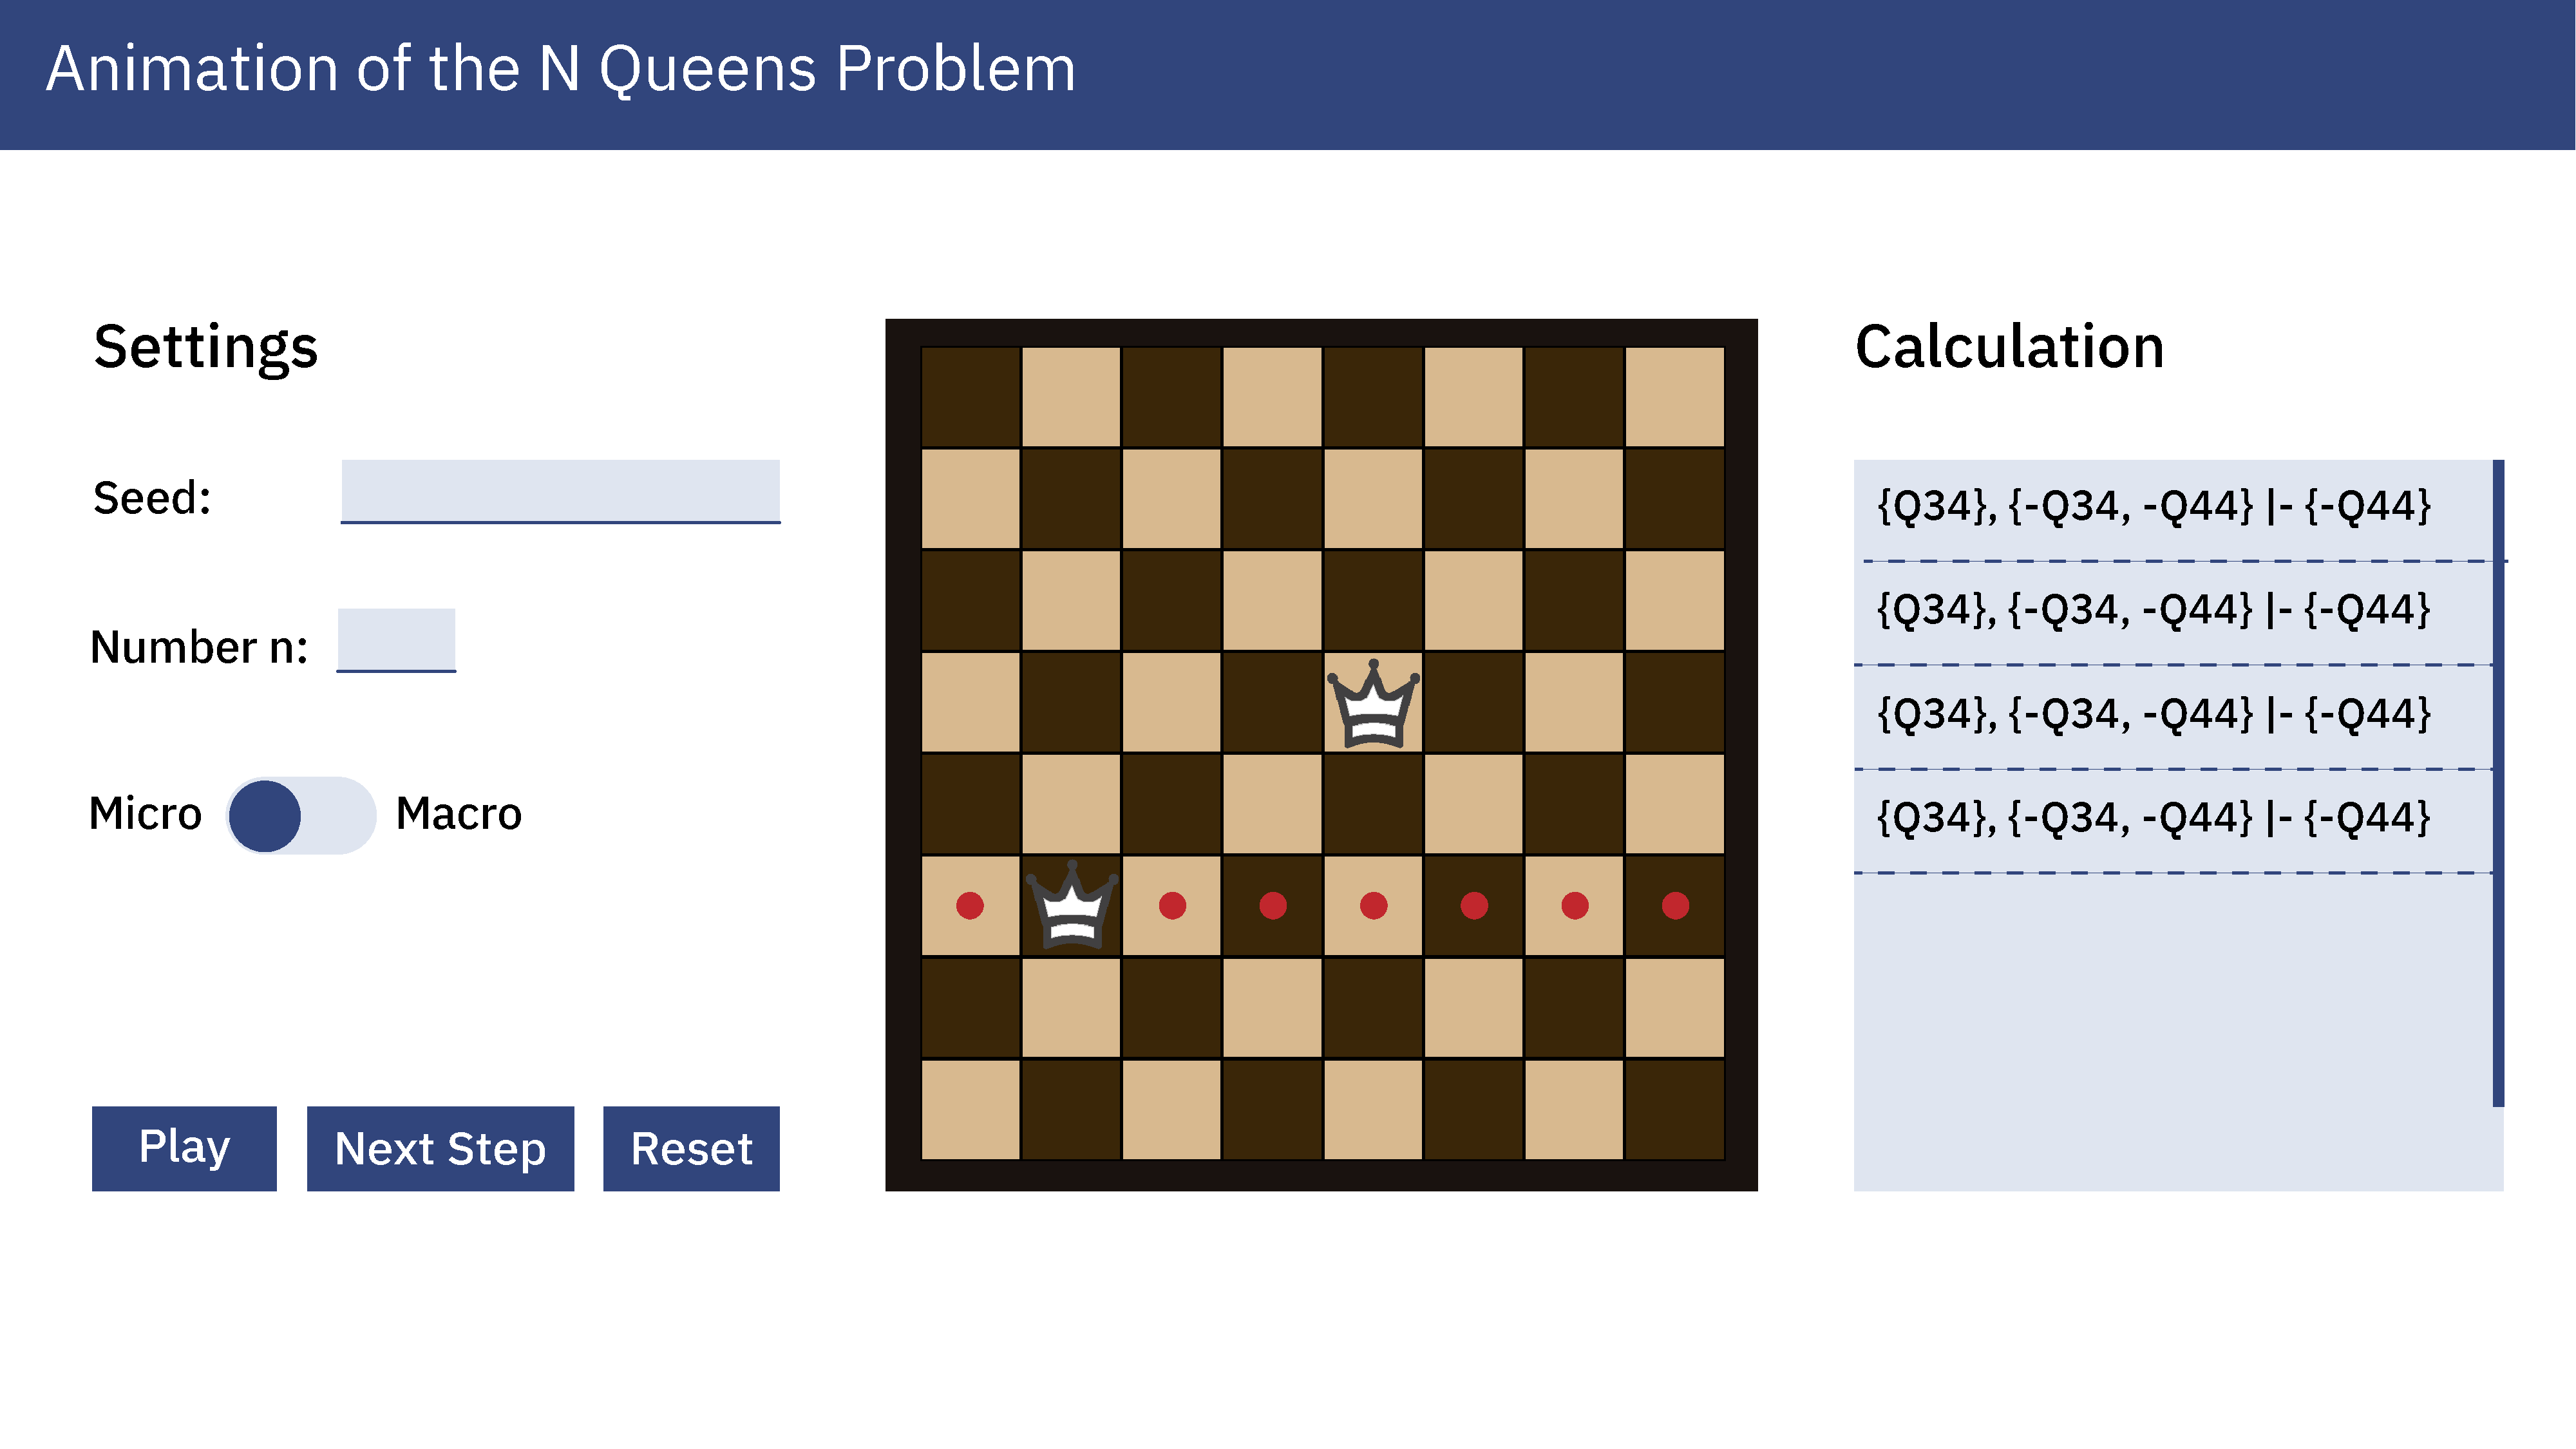
\includegraphics[width=\textwidth]{img/Design_N_Queens}
  \caption{Final Design Sketch for User Interface}
  \label{fig:design}
\end{figure}
Der Header dabei dient als Blickfang, so dass sofort das Thema der Website klar und verständlich heraussticht. Dabei nimmt er die Funktion einer Überschrift ein. 
\\
Darunter wird die Benutzeroberfläche visuell in drei Teile eingeteilt. Dabei befindet sich in der Mitte das Schachbrett, da hier die Hauptanimation stattfindet und somit der Mittelpunkt bilden sollte. Es fängt sofort den Blick der Nutzer ein und leitet sie auf das Hauptgeschehen weiter. 
\\
Links davon befinden sich die Einstellungen zur Animation und Durchführung des Algorithmus. Es entsteht ein natürlicher Lesefluss von links nach rechts, der von den Einstellungen über das Schachbrett hin zu den Kalkulationen geht. Der Nutzer wird inutitiv und selbsterklärend durch das System navigiert, ganz ohne auffällige Steuerungselemente. Die Einstellungen beinhalten dabei nur die wichtigsten Elemente, mit denen die Animation eingestellt werden kann. Dadurch wirkt es nirgends überladen, sondern übersichtlich und strukturiert. Darunter befinden sich die Buttons zur Steuerung der Animation. Je nach Situation wird die Funktionalität dieser angepasst. In diesem Entwurf nehmen die Einstellungen einen festen Platz auf der Oberfläche ein, es gab jedoch durchaus auch die Idee, die Settings in ein aufklappbares sidemenu umzusetzen. Dagegen sprach jedoch die Tatsache, dass der Nutzer dauerhaft mit den Steuerbuttons interagieren muss und aufklappbare Menüs sich nur für einmalige Interaktionen wie beispielsweise die Navigation durch eine Seite anbietet. 
\\
Auf der rechten Seite der Benutzeroberfläche befindet sich die Kalkulation, die den mathematischen Hintergrundprozess in einzelnen Schritten aufzeigt. Die einzelnen Schritte werden dabei in einer scrollbaren Box angezeigt. Ob das oberste Element immer oben bleibt oder die neueren darüber gelegt werden, ist im Design selbst nicht festgelegt.
\\
Wichtig ist, dass alle Komponenten schlüssig miteinander sind. Das bedeutet, dass die Positionierung, der Abstand und das Alignment konsistent sind. Nur dann entsteht am Ende ein stimmiges Gesamtbild. Auch die Farben wurden so gewählt, dass sie beruhigend und in einem einheitlichen Ton, aber mit unterschiedlichen Sättigungen erscheinen. Damit wirkt die Oberfläche harmonisch und nicht überladen. Das Braun des Schachbretts passt sehr gut zum Blauton in der Umgebung und sticht als einzig anderer Farbton aus der Masse hervor. Dieses Farbschema galt jedoch nur zu Demonstrationszwecken und Orientierung. Es kann im Laufe der Implementierung angepasst werden und durch ein passenderes Set ersetzt werden. Ein gut strukturiertes und übersichtliches Layout ist entstanden, welches für die Nutzer leicht verständlich und einfach zu benutzen ist.
    % !TeX root = ./documentation.tex

\chapter{Implementation}
\label{ch:implementation}
As mentioned before in the chapter \ref{ch:tecBasics} we will be using Node.js with Parcel as a module bundler. This way we can use Node.js modules and build an HTML page that does not require a Node.js server running in the background, making it portable and executable without any prerequisites except for a browser. The implementation in JavaScript will be object orientated approach using the with ECMAScript 2015 introduced class syntax, which will make it more pleasing for the eye and less confusing.
% Class Syntax https://developer.mozilla.org/en-US/docs/Web/JavaScript/Reference/Classes

\section{Util Class}
\label{sec:impUtil}

\section{Implementing the Algorithm of Davis \& Putnam}
\label{sec:impDavisPutnam}
The original algorithm of Davis \& Putnam is recursive and so are most of its implementations. If you were to calculate everything at one till you find a possible solution or the response that the given problem can not be satisfied, then a recursive implementation is not an issue. For our purposes, which is the visualization of the algorithm as it solves the given problem step by step, we prefer to use a iterative implementation. Because an iterative implementation can be paused at any point depending on how its implemented.

One of the challenges here is the double recursive call of the algorithm

\subsection{Davis Putnam Class}

\subsection{Davis Putnam Consumer Class}

\subsection{Davis Putnam Worker Class}

\section{Implementing N-Qeens Problem}
\label{sec:impQueens}

\subsection{Queens Clauses Function}

\subsection{Chessboard Class}

\section{Implementing User Interaction}
\label{sec:impUI}

\subsection{HTML Document}

\subsection{CSS Document}

\subsection{Frame Class}
    % !TeX root = ./documentation.tex

\chapter{Prospect}
\section{Evaluation}
\section{Conclusion}
\section{Outlook} %TODO if there is something....
% ------------------------------------------------------------------

\label{lastpage}

% Neue Seite
\cleardoublepage

% Backmatter mit normalem Zeilenabstand setzen
\singlespacing

% Römische Ziffern für die "Back-Matter", fortlaufend mit "Front-Matter"
\pagenumbering{roman}
\setcounter{page}{\value{frontmatterpage}}

% Abkürzungsverzeichnis
\addchap{\dhbwabbreviations}
%\begin{acronym}
\acro{ABK}{Abkürzung}
\acro{ACM}{Association of Computing Machinery}
\acro{PDF}{Portable Document Format}
\acro{IEEE}{Institute of Electrical and Electronics Engineers}
\acro{ISO}{International Organization for Standardization}
%%%%%%%%%%%%%%%%%%%%%%%%%%%%%%%%%%%%%%%%%%%%%%%%%%%%%%%%%%%%%%%%
%a

%b

%c

%d

%e

%f

%g

%h

%i

%j

%k

%l

%m

%n

%o

%p

%q

%r

%s

%t

%u

%v

%w

%x

%y

%z

\end{acronym}



% Tabellenverzeichnis erzeugen
\cleardoublepage
\phantomsection
\addcontentsline{toc}{chapter}{\dhbwlistoftables}
\listoftables

% Abbildungsverzeichnis erzeugen
\cleardoublepage
\phantomsection
\addcontentsline{toc}{chapter}{\dhbwlistoffigures}
\listoffigures

%% Listingverzeichnis erzeugen
%\cleardoublepage
%\phantomsection
%\addcontentsline{toc}{chapter}{\dhbwlistings}
%\lstlistoflistings

% Literaturverzeichnis erzeugen
\begin{flushleft}
\printbibliography
\end{flushleft}

% Index ausgeben. Wenn Sie keinen Index haben, entfernen Sie einfach
% diesen Teil.
\cleardoublepage
\phantomsection
\addcontentsline{toc}{chapter}{\dhbwindex}
\printindex

% Anhang. Wenn Sie keinen Anhang haben, entfernen Sie einfach
% diesen Teil.
%\appendix
%\input{tex/anhang-a}
%\input{tex/anhang-b}

\end{document}





%\documentclass{report}
%\usepackage[utf8]{inputenc}
%\usepackage[english]{babel}
%\usepackage{graphicx}
%\usepackage{a4wide}
%%\usepackage{epsfig}
%
%\usepackage{hyperref}
%\usepackage[all]{hypcap}
%\hypersetup{
%	colorlinks = true,
%	linkcolor  = blue,
%	citecolor  = red,
%    filecolor  = gold,
%    urlcolor   = [rgb]{0.5, 0.0, 0.5},
%	pdfborder  = {0 0 0} 
%}
%
%\usepackage{fancyhdr}
%\usepackage{lastpage}
%
%\renewcommand*{\familydefault}{\sfdefault}
%
%\pagestyle{fancy}
%
%\fancyfoot[C]{--- \thepage/\pageref{LastPage}\ ---}
%
%\fancypagestyle{plain}{
%    \fancyhf{}
%    \fancyfoot[C]{--- \thepage/\pageref{LastPage}\ ---}
%    \renewcommand{\headrulewidth}{0pt}
%}
%
%\renewcommand{\chaptermark}[1]{\markboth{\chaptername \ \thechapter.\ #1}{}}
%\renewcommand{\sectionmark}[1]{\markright{\thesection. \ #1}{}}
%\fancyhead[R]{\leftmark}
%\fancyhead[L]{\rightmark}
%
%\author{Koen Loogman \& Jessica Roth}
%%\title{\epsfig{file=dhbw-logo.eps, scale=1.0}\\[0.3cm]
%\title{ 
%        Animation N Queens Problem in Javascript\\[0.3cm]
%        DHBW Mannheim}
%\date{\today}
%

%
%
%\begin{document}
%
%    \maketitle
%    \tableofcontents
%
%    % !TeX root = ./documentation.tex

\chapter{Introduction}
\section{Motivation}
\section{Objective of the work}
Die Aufgabenstellung dieser Studienarbeit handelt von der Animation des Davis Putman Algorithmus anhand des N Damen Problems mit der Hilfe von Javascript. Dabei werden mehrere Kriterien definiert, die diese Animation erfüllen muss, da sie vor allem zur Visualisierung und zur genaueren anschaulichen Verdeutlichung beziehungsweise Erklärung des Algorithmus dient. Die genauen Anforderungen werden im Laufe dieser Arbeit genauer spezifiziert und am Ende am finalen Produkt evaluiert. Der Hauptteil dieser Arbeit handelt deshalb von der Konzeption und der Implementierung dieser Aufgabenstellung.
%TODO Koen: Fällt dir noch etwas dazu ein?
\section{Structure of the report}
Um die Navigation durch diese Arbeit zu erleichtern, wird im folgenden Abschnitt einen kurzen Blick in die Struktur dieser Arbeit geworfen. 
\\
Im nächsten Kapitel werden die mathematischen Grundlagen zum Davis Putman Algorithmus und des N Damen Problems geschaffen. Dabei handelt es sich vor allem um die logischen Zusammenhänge und der mathematisch korrekten Definition des zu lösenden Problems. 
\\
Darauffolgend wird im dritten Kapitel ein allgemeiner Überblick zu den verwendeten Bibliotheken und Technologien gegeben und Hintergrundinformationen geliefert, aus welchen Gründen bestimmte Technologien bevorzugt beziehungsweise ausgewählt wurden.
\\
Im vierten Abschnitt dieser Arbeit wird die Konzeption des Programms genauer betrachtet. Vor allem handelt es von der allgemeinen Architektur und dem erstellten Layout Design, das als Vorlage für die Implementierung der Benutzeroberfläche dient. Eingeleitet wird das Kapitel durch das Spezifizieren der Anforderungen für das Programm, die eine zentrale Rolle in der Evaluation am Ende spielen.
\\
Im fünften Kapitel wird nun Schritt für Schritt durch die fertige Implementierung geleitet und der Aufbau des Programms genauer erläutert. Dabei wird durch die unterschiedlichen Komponenten und Klassen geführt und dabei ihre Funktion genauer erläuert.
\\
Das letzte Kapitel wird mit der Evaluation der Anforderungen begonnen. Dies dient vor allem dazu, um zu schauen, ob das Programm alle Kriterien erfüllt und zu Ende als erfolgreich erfüllt angesehen werden kann. Danach folgt ein zusammenfassendes Fazit und ein Ausblick, wie das Programm zukünftig weiterentwickelt oder anders eingesetzt werden könnte.
%    % !TeX root = ../documentation.tex

% Davis Putnam in own word

\chapter{Scientific Basics}
% cSpell:disable
% Das Ziel dieser Arbeit besteht in der Visualisierung des Davis Putman Algorithmus, der das sogenannte N damen Problem lösen soll. Dafür muss zuerst ein allgemeines Verständnis zu diesem Algorithmus und dem mathematischen Problem geschaffen werden. In diesem Kapitel wird aus diesem Grund dieses fundamentale Wissen zusammengefasst, um eine Basis für die weiterführende Entwicklung zu schaffen. Dafür spielt unter anderem die Deklarierung des mathematischen Problems eine Rolle, damit dieses vom Davis Putman Algorithmus gelöst werden kann.
% cSpell:enable
The purpose of this work is to visualize the Davis Putman algorithm solving the so-called \textit{N-Queens Problem}. 
Therefore a general understanding of this algorithm and the mathematical problem has to be created.

This chapter summarizes the fundamental knowledge that is needed in order to create a basis for further development. 
%TODO: rephrase following sentence:
Among other things, the definition of the mathematical problem plays a role here, so that it can be solved by the Davis Putman algorithm.

\section{The Algorithm of Davis \& Putnam}
% cSpell:disable
% Der Davis Putman Algorithmus ist ein Verfahren zur Berechnung einer Lösung von aussagelogischen Klauselmengen. Bei sehr kleinen Klauselmengen kann dies leicht bestimmt werden, wie in den zwei folgenden Beispielen zu sehen ist.
% cSpell:enable
The Davis Putman algorithm is a method for calculating a solution a set of propositional clauses. With very small clause sets this can be easily determined, as can be seen in the following two examples.
\\
\hspace*{1.3cm} 
$K_1 = \bigl\{\; \{r\},\; \{\neg s\},\; \{t\},\; \{\neg u\}, \; \{\neg v\} \;\bigr\}$ 
\\[0.2cm]
$K_1$
% cSpell:disable
%kann auch als aussagelogische Formel geschrieben werden.
% cSpell:enable
can also be written as a propositional logic formula.
\\[0.2cm]
\hspace*{1.3cm}
$r \land \neg s \land t \land \neg u \land \neg v$.
\\[0.2cm]
% cSpell:disable
% Es ist erkennbar, dass diese Formel lösbar ist, indem $r$ und $t$ \enquote{wahr} und $s$, $u$ und $v$ den Wert \enquote{falsch} haben. Als Gegenbeispiel dazu ist $K_2$ zu betrachten.
% cSpell:enable
It is recognizable that this formula is solvable by $r$ and $t$ \enquote{true} and $s$, $u$ and $v$ having the value \enquote{false}.
As a counter example $K_2$ is to be considered.
\\
\hspace*{1.3cm}
$K_2 = \bigl\{\; \{r\},\; \{\},\; \{t\} \;\bigr\}$ 
\\[0.2cm]
$K_2$ can also be written as a propositional logic formula.
\\[0.2cm]
\hspace*{1.3cm}
$r \land \bot \land t$.
\\[0.2cm]
% cSpell:disable
% Eine leere Klammer bedeutet in der Aussagelogik ein Falsum, wodurch $K_2$ unerfüllbar ist. Bei sehr großen Klauselmengen ist es meist nicht mehr auf dem ersten Blick zu sehen, so dass Algorithmen wie dieser eingesetzt werden. Doch um nun einen Schritt tiefer setzen zu können, müssen zwei Definitionen zuvor eingeführt werden.
% cSpell:enable
The empty set in the set of clauses $K_2$ is interpreted as a $\bot$ in the propositional logic, making it impossible to satisfy $K_2$. It is possible to satisfy smaller sets of less complex clauses by first glance, but it gets more difficult for larger and complexer sets of clauses. For these algorithms like the Davis Putman algorithm are used.
% TODO: rephrase following sentence:
But to be able to set a step lower, two definitions have to be introduced first. \cite{Zhang2000}

\paragraph{Unit clause}
% cSpell:disable
% Eine Klausel $C$ ist eine Unit-Klausel, wenn diese nur aus einem Literal, also aus einer Aussagevariablen besteht.
% cSpell:enable
A clause $C$ is a unit clause if it consists of only one literal, i.e. a variable or a negated variable.

\paragraph{trivial clause sets}
% cSpell:disable
% Eine triviale Klauselmenge kann nur vorkommen, wenn einer der beiden Fälle eintritt.
% cSpell:enable
A trivial set of clauses can only occur if one of the following two cases occurs.

\begin{enumerate}
% cSpell:disable
% $K$ enthält die leere Klausel und ist somit unerfüllbar
% cSpell:enable
\item A set of clauses $K$ contains the empty set and is therefore unsatisfiable
% cSpell:disable
% Die Unit-Klauseln beinhalten immer verschiedene Aussagevariablen, so dass entweder nur die Klausel $\{p\}$ oder $\{\neg p\}$ vorkommen kann. Ist dies der Fall, kann eine Lösung für die Klauselmenge bestimmt werden.
% cSpell:enable
\item The unit clauses always contain different statement variables, so that only the clause $\{p\}$ or $\{\neg p\}$ can occur. If this is the case, a solution for the clause set can be determined.
\end{enumerate}

% cSpell:disable
% Damit einer dieser beiden Fälle nun eintreten kann, müssen die Klauselmengen mit der Hilfe folgender drei Möglichkeiten so vereinfacht werden, dass diese nur aus Unit-Klauseln bestehen.
% cSpell:enable
In order for one of these two cases to occur, the clause sets must be simplified with the help of the following three options so that they consist only of unit clauses.

\begin{enumerate}
\item Cut Rule 
\item Subsumption
\item Case Differentiation
\end{enumerate}

% TODO: continue here
\subsection{Simplification with the Cut Rule} 
To simplify a set of clauses $K$ with $C_1 \cup \{\; p\; \}\, C_2 \cup \{\; \neg p\; \} \in K$ the cut rule can be used. Lets say we have two clauses $C_1$, $C_2$ and a variable $p$. A typical application of the cut rule is.
\\
\hspace*{1.3cm}
$\dfrac{C_1 \cup \{\; p\; \} \;\;\;\;\;\; C_2 \cup \{\; \neg p\; \}}{C_1 \cup C_2}$
\\[0.2cm]
In this case the result clause will in general have more literals than $C_1 \cup \{\; p\; \}$ or $C_2 \cup \{\; \neg p\; \}$ alone. Because if the clause $C_1 \cup \{\; p\; \}$ contains $m + 1$ literals and $C_1 \cup \{\; p\; \}$ contains $n + 1$ literals, then the union $C_1 \cup C_2$ can have upto $m + n$ literals in total. In general $m + n$ is bigger than $m + 1$ or $n + 1$. The clause can be smaller than previously if both sets contain the same literals, but it is only granted to be smaller if $m = 0 \lor n = 0$. This is the case for unit clauses. Therefore we will only allow the use of the cut rule if one of the clauses is a unit clause. These cuts will be called unit cuts. To be able to do those unit cuts with a unit clause $\{\; l\; \}$ on all clauses of a set of clauses $K$, we define the function
\\
\hspace*{1.3cm}
$\texttt{unitCut}: 2^{K} \times L \to 2^{K}$
\\[0.2cm]
so that for a set of clauses $K$ and a literal $l$ the function $\texttt{unitCut}(K,\; l)$ will simplify the set of clauses as much as possible by using unit cuts:
\\
\hspace*{1.3cm}
$\texttt{unitCut}(K,\; l) = \{\; C \setminus \{\; \neg l\; \}\; |\; C \in K\; \}$
\\[0.2cm]
The result set of clauses will have the same amount of clauses as $K$. Only the clauses $C \in K$ where $\neg l \in C$ were affected and got that element removed. \cite{Stroetman2019}

\subsection{Simplification with Subsumption}
For further simplification of the set of clauses we will use subsumption. The idea is simple and can be shown with the following example:
\\
\hspace*{1.3cm}
$K = \{\; \{\; l,\; p,\; \neg q \;\},\; \{\; l\; \}\; \} \cup M$
\\[0.2cm]
It is clear that the clause $\{\; l\; \}$ implies the clause $\{\; l,\; p,\; \neg q \;\}$, because if $\{\; l\; \}$ is satisfied, then $\{\; l,\; p,\; \neg q \;\}$ will be satisfied too. That's because
\\
\hspace*{1.3cm}
$\models l \to l \lor p \lor \neg q$
\\[0.2cm]
is given. With that in mind we can say that we can subsume a clause $C$ with a unit clause $U$ if $U \subseteq C$. That means if we have a set of clauses $K$ with $C \in K \land U \in K$ and $U$ can subsume $C$, we can remove the clause $C$ from $K$ to reduce its size. We define a function
\\
\hspace*{1.3cm}
$\texttt{subsume}: 2^{K} \times L \to 2^{K}$
\\[0.2cm]
that receives a set of clauses $K$ and a literal $l$. It will simplify $K$ by subsuming with the unit clause $\{\; l\; \}$:
\\
\hspace*{1.3cm}
$\texttt{subsume}(K,\; l) = \{\; C \in K\; |\; l \notin C\} \cup \{\{\; l\; \}\}$
\\[0.2cm]
We have to add the unit clause to the set of clauses, because $l \in U$ is the case. Resulting in $U$ being removed from $K$ at first too. \cite{Stroetman2019}

\subsection{Simplification with Case Differentiation}
% cSpell:disable
% Die Basis für das Prinzip der Fallunterscheidung bildet folgender Satz.
% cSpell:enable
The following theorem forms the basis for the principle of case differentiation.

\paragraph{Theorem}
% cSpell:disable
% Die Klauselmenge K ist genau dann erfüllbar, wenn die Klausel $K \cup \bigl\{\{p\}\bigr\}$ oder $K \cup \bigl\{\{\neg p\}\bigr\}$ erfüllbar ist.
% cSpell:enable
The set of clauses $K$ can only be satisfied if $K \cup \bigl\{\{p\}\bigr\}$ or $K \cup \bigl\{\{\neg p\}\bigr\}$ can be satisfied.

% cSpell:disable
% Für die Vereinfachung wird zu Beginn also eine Aussagenvariable p ausgewählt, die in der Klauselmenge vorkommt. Danach werden die beiden oben genannten Klauselmengen gebildet und versucht, für eine der beiden eine Lösung zu finden. Ist dieser Versuch erfolgreich, ist das Ergebnis automatisch die Lösung von $K$. Falls keine gefunden wird, ist $K$ unlösbar.
% TODO: Keine Ahnung ob hier Beweis einfügen soll
% cSpell:enable
For simplification, a statement variable p is selected at the beginning, which occurs in the clause set. Then the two clause sets mentioned above are formed and an attempt is made to find a solution for one of them. If this attempt is successful, the result is automatically a solution of $K$. If none is found, $K$ is unsolvable.

\subsection{The Davis-Putnam Method}
% cSpell:disable
% Durch die Wissensgrundlage, die zuvor geschaffen wurde, ist es nun möglich, das Vorgehen des Davis Putman Algorithmus zu skizzieren. Mit der Hilfe der Schnittregel und der Subsumption wird die Klauselmenge $K$ soweit es möglich ist, vereinfacht. Falls bereits nach diesem Schritt $K$ trivial ist, ist das Verfahren beendet. Andernfalls wird eine aussagelogische Variable p ausgewählt, die in K vorkommt. Dann wird rekursiv versucht, die Klauselmenge $K \cup \bigl\{\{p\}\bigr\}$ zu lösen, um eine Lösung für K zu finden. Wenn auch hier keine Lösung gefunden wurde, wird dasselbe mit dem negierten $p$ versucht. Scheitert auch dieser Versuch, ist K unlösbar.
% cSpell:enable
The theoretical foundation that was previously created now makes it possible to sketch the procedure of the Davis Putman algorithm. With the help of the intersection rule and the subsumption, the clause set $K$ is simplified as far as possible. If already after this step $K$ is trivial, the procedure is finished. Otherwise a statement logical variable p is selected, which occurs in K. Then a recursive attempt is made to solve the clause set $K \cup \bigl\{\{p\}\bigr\}$ in order to find a solution for K. If no solution was found here either, the same is tried with the negated $p$. If this attempt also fails, K is unsolvable.\cite{Zhang2000}, \cite{Stroetman2019}
% TODO: find more sources

% TODO: nicely format
\begin{listing}[ht]
function Satisfiable( clause set $S$ ) return boolean\\
  /* unit propagation */\\
  repeat for each unit clause $L$ in $S$ do\\
    /* unit subsumption */\\
    delete from $S$ every clause containing $L$\\
    /* unit resolution */\\
    delete $L$ from every clause of $S$ in which it occurs\\
  od\\
  if $S$ is empty then\\
    return true\\
  else if a clause becomes $\{\}$ in $S$ then\\
    return false\\
  fi\\
  until no further changes result\\
  /* splitting */\\
  choose a literal $L$ occurring in $S$\\
  if Satisfiable ($S \cup \{\{\neg L\}\}$) then\\
    return true\\
  else if Satisfiable ($S \cup \{\{L\}\}$) then\\
    return true\\
  else\\
    return false\\
  fi\\
end function
  \caption{A simple Davis–Putnam algorithm \cite{Zhang2000}}
  \label{listing:1}
\end{listing}  


\section{N Queens Problem}
% cSpell:disable
% Das n Königinnen Problem ist das verallgemeinerte mathematische Problem bezogen auf ein Schachbrett, dass n \times n Felder besitzt. Ein spezielles Beispiel dazu wäre das 8 Damen Problem, welches auf dem standardisierten Schachbrett abgebildet wird. Allgemein handelt das Problem davon, n Damen auf einem n \times n Schachbrett so zu platzieren, dass keine in ihrem Zug behindert werden würde. Eine Königin in einem normalen Schachspiel kann sowohl diagonal, als auch vertikal und horizontal ihre Züge ziehen. Dieses Zugmuster kann in Figure \ref{fig:queens-problem} genauer angeschaut werden. Zusammengefasst heißt dies also, dass immer nur eine Dame auf ihrer vertikalen, horizontalen und diagonalen Linie sein darf, um sich nicht gegenseitig zu behindern. Dabei wird in diesem Problem davon ausgegangen, dass jede Dame jede andere angreifen kann und die Feldfarben ignoriert werden. 
% cSpell:enable
The n queen problem is the generalized mathematical problem related to a chessboard that consists of $n \times n$ squares. A special example would be the 8 queens problem, which is related to the standardized chessboard. In general, the problem is to place n queens on an $n \times n$ chessboard so that none would be obstructed in their turn. A queen in a normal game of chess can move diagonally, vertically and horizontally. This move pattern can be seen in Figure \ref{fig:queens-problem}. In summary, this means that there is only one queen allowed on her vertical, horizontal and diagonal line at a time so that they do not interfere with each other. In this problem it is assumed that any queen can attack any other queen and the field colors are ignored. This problem can be solved by several algorithms such as the Davis Putman algorithm. \cite{Bell2009}, \cite{Watkins2012}, \cite[146\psq]{Nudelman1995}, \cite{Stroetman2019}

\begin{figure}[!ht]
  \centering
  \setlength{\unitlength}{1.0cm}
  \begin{picture}(10,9)
    \thicklines
    \put(1,1){\line(1,0){8}}
    \put(1,1){\line(0,1){8}}
    \put(1,9){\line(1,0){8}}
    \put(9,1){\line(0,1){8}}
    \put(0.9,0.9){\line(1,0){8.2}}
    \put(0.9,9.1){\line(1,0){8.2}}
    \put(0.9,0.9){\line(0,1){8.2}}
    \put(9.1,0.9){\line(0,1){8.2}}
    \thinlines
    \multiput(1,2)(0,1){7}{\line(1,0){8}}
    \multiput(2,1)(1,0){7}{\line(0,1){8}}
    \put(4.15,6.15){{\chess Q}}
    \multiput(5.25,6.5)(1,0){4}{\vector(1,0){0.5}}
    \multiput(3.75,6.5)(-1,0){3}{\vector(-1,0){0.5}}
    \multiput(5.25,7.25)(1,1){2}{\vector(1,1){0.5}}
    \multiput(5.25,5.75)(1,-1){4}{\vector(1,-1){0.5}}
    \multiput(3.75,5.75)(-1,-1){3}{\vector(-1,-1){0.5}}
    \multiput(3.75,7.25)(-1,1){2}{\vector(-1,1){0.5}}
    \multiput(4.5,7.25)(0,1){2}{\vector(0,1){0.5}}
    \multiput(4.5,5.75)(0,-1){5}{\vector(0,-1){0.5}}
  \end{picture}
  \vspace*{-1.0cm}
  \caption{The 8-Queens-Problem \cite{Stroetman2019a}} 
  \label{fig:queens-problem}
\end{figure}
%    % !TeX root = ./documentation.tex

% Javascript und verwendete Libraries

\chapter{Technical Basics}
%    % !TeX root = ./documentation.tex

\chapter{Implementation}
\label{ch:implementation}
As mentioned before in the chapter \ref{ch:tecBasics} we will be using Node.js with Parcel as a module bundler. This way we can use Node.js modules and build an HTML page that does not require a Node.js server running in the background, making it portable and executable without any prerequisites except for a browser. The implementation in JavaScript will be object orientated approach using the with ECMAScript 2015 introduced class syntax, which will make it more pleasing for the eye and less confusing.
% Class Syntax https://developer.mozilla.org/en-US/docs/Web/JavaScript/Reference/Classes

\section{Util Class}
\label{sec:impUtil}

\section{Implementing the Algorithm of Davis \& Putnam}
\label{sec:impDavisPutnam}
The original algorithm of Davis \& Putnam is recursive and so are most of its implementations. If you were to calculate everything at one till you find a possible solution or the response that the given problem can not be satisfied, then a recursive implementation is not an issue. For our purposes, which is the visualization of the algorithm as it solves the given problem step by step, we prefer to use a iterative implementation. Because an iterative implementation can be paused at any point depending on how its implemented.

One of the challenges here is the double recursive call of the algorithm

\subsection{Davis Putnam Class}

\subsection{Davis Putnam Consumer Class}

\subsection{Davis Putnam Worker Class}

\section{Implementing N-Qeens Problem}
\label{sec:impQueens}

\subsection{Queens Clauses Function}

\subsection{Chessboard Class}

\section{Implementing User Interaction}
\label{sec:impUI}

\subsection{HTML Document}

\subsection{CSS Document}

\subsection{Frame Class}
%    % !TeX root = ./documentation.tex

\chapter{Prospect}
\section{Evaluation}
\section{Conclusion}
\section{Outlook} %TODO if there is something....
%
%    \bibliographystyle{alpha}
%
%    \bibliography{cs}
%
%\end{document}